\documentclass{beamer}
\usetheme{CambridgeUS}
\useoutertheme{aria}

\setbeamertemplate{blocks}[rounded][shadow=true]
\setbeamertemplate{items}[circle]

%\setbeamertemplate{frametitle}[default][none]


\definecolor{aria-green}{RGB}{146, 200, 62}
\definecolor{aria-gray}{RGB}{85, 80, 80}

\definecolor{darkred}{rgb}{0.8,0,0}

\setbeamercolor{section in toc}{fg=black,bg=white}
\setbeamercolor{alerted text}{fg=darkred!80!gray}
\setbeamercolor*{palette primary}{fg=aria-green!60!black,bg=gray!30!white}
\setbeamercolor*{palette secondary}{fg=aria-green!70!black,bg=gray!15!white}
\setbeamercolor*{palette tertiary}{bg=aria-green!80!black,fg=gray!10!white}
\setbeamercolor*{palette quaternary}{fg=aroa-green,bg=gray!5!white}

\setbeamercolor*{sidebar}{fg=aria-green,bg=gray!15!white}

\setbeamercolor*{palette sidebar primary}{fg=aria-green!10!black}
\setbeamercolor*{palette sidebar secondary}{fg=white}
\setbeamercolor*{palette sidebar tertiary}{fg=aria-green!50!black}
\setbeamercolor*{palette sidebar quaternary}{fg=gray!10!white}

\setbeamercolor{titlelike}{parent=palette primary,fg=aria-green}
\setbeamercolor{frametitle}{bg=aria-green,fg=white}
\setbeamercolor{frametitle right}{bg=gray!60!white}

\setbeamercolor*{separation line}{}
\setbeamercolor*{fine separation line}{}

\setbeamercolor*{structure}{aria-green}
\setbeamercolor*{block title}{bg=aria-green,fg=white}

\usepackage[utf8x]{inputenc}
\usepackage{tabularx}
\usepackage[romanian]{babel}
\usepackage{natbib}
\usepackage{bibentry}
\usepackage{amsmath}
\usepackage{mathtools}
\usepackage{algorithm}
\usepackage{algorithmic}
\usepackage{graphicx}
\usepackage{caption}
\usepackage{subcaption}
\usepackage{hyperref}

%\usepackage[framed,numbered,autolinebreaks,useliterate]{mcode}
\usepackage{tikz}
\usetikzlibrary{arrows}
\tikzstyle{block}=[draw opacity=0.7,line width=1.4cm]


\title[Modele Markov Ascunse]{Modele Markov Ascunse}

%
%\subtitle{De la Teorie la Aplicații}
%
\author[ARIA]{ARIA}
%
%\institute[AI-MAS]{Asociația Română pentru Inteligență Artificială}

%% TODO de pus frumos titlurile secțiunilor

%% Autori: Alexandru Sorici, Tudor Berariu
%% Data: Noiembrie 2012

\titlegraphic{
  
\includegraphics[height=.25\textheight]{graphics/branding/aria-logo-small-white.png}
}

%% Numele algoritmului
\floatname{algorithm}{Algoritmul}

%% comandă care trage o linie orizontală (80% din spațiu)
\newcommand{\horiline}{
  \vspace*{-.75em} \begin{center} \begin{tabularx}{.8\linewidth}{
        l } \hline
    \end{tabularx}
  \end{center}
  \vspace*{-.75em}
}

%% comandă pentru frame-uri goale
\newcommand{\dummyframe}{
  \begin{frame}
    \frametitle{De înlocuit} 
    :) 
  \end{frame}
}


%% afișează cuprinsul înainte de fiecare subsecțiune
\AtBeginSubsection[] {
  %\renewcommand\Switch{0}
  \begin{frame}{Outline}
    \tableofcontents[currentsection,currentsubsection,hideallsections]
  \end{frame}
  %\renewcommand\Switch{1}
}



\begin{document}
%\maketitle

\begin{frame}[t]
	\begin{center}
		\Large{3 chestii tari despre ARIA}
	\end{center}%
	\pause
	
	\begin{columns}
		\column{0.60\textwidth}
			\begin{center}
				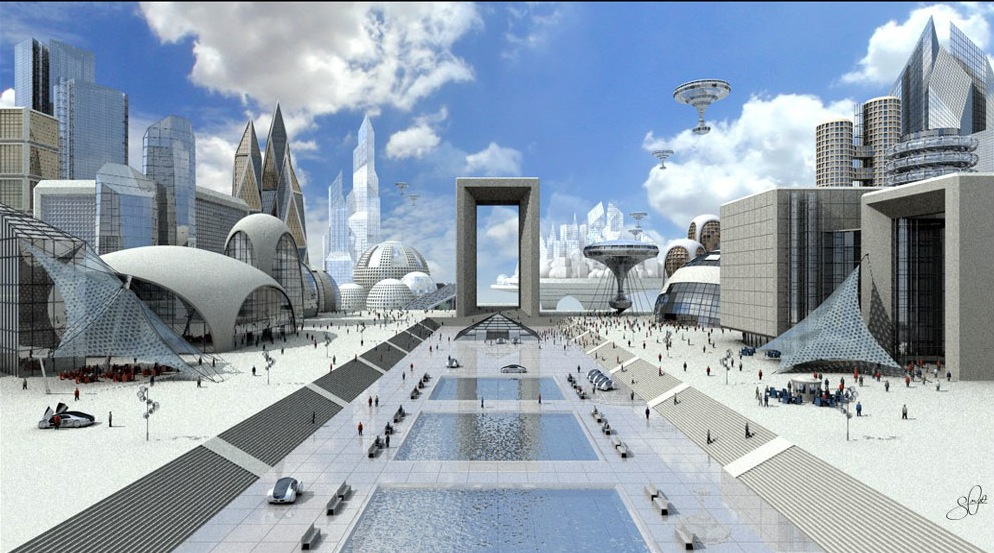
\includegraphics[width=0.8\textwidth]{graphics/intro/rlandri}\\%
				\small{The White City of R'Landri}
			\end{center}
			\pause
		\column{0.40\textwidth}
			\textbf{ARIA Bulletin}%
			\vspace*{0.25em}
			\begin{itemize}
				\item 2.5 articole / săpt.
				\item \small{\url{http://bit.ly/UWR65L}}
				\pause
				\item \small{\url{add@aria-romania.org}}
			\end{itemize}
	\end{columns}
	\pause	
	
	\begin{center}
		
\includegraphics[width=0.45\textwidth]{graphics/intro/aria-hackathon}%
	\end{center}
\end{frame}

\begin{frame}[t]
	\begin{center}
		\LARGE{Asociația Română pentru Inteligență Artificială}
	\end{center}%
	\begin{itemize}
		\item 9 aprilie 2011
		\item 38 membri, 9 universități
	\end{itemize}

	
	\begin{center}
	\begin{columns}[h]
			\column{0.25\textwidth}
			\column{0.25\textwidth}
			\centering{
\includegraphics[width=0.45\textwidth]{graphics/intro/upb-logo}}%

			\column{0.25\textwidth}
			\centering{
\includegraphics[width=0.45\textwidth]{graphics/intro/racai-logo}}%
			\column{0.25\textwidth}

	\end{columns}
	\end{center}%
	
	\begin{center}
		
\includegraphics[width=0.25\textwidth]{graphics/intro/aquasoft-logo}%
	\end{center}%

	\begin{columns}[h]
			\column{0.4\textwidth}
			\hfill 
\includegraphics[width=0.6\textwidth]{graphics/intro/eccai-logo}%
			\column{0.6\textwidth}
			\small{\textbf{European Coordinating}} \hfill\\%
			\small{\textbf{Commitee for Artificial Intelligence}} \hfill%
	\end{columns}
\end{frame}

\begin{frame}[t]
	\begin{center}
		\huge{ARIA Education}\\%
	\end{center}
	
	\begin{itemize}
		\setlength{\itemindent}{3.6em}
		\item \Large{HMMs: from Theory to Applications}
	\end{itemize}

	
	\setlength{\itemindent}{0em}
	\begin{center}
		
\includegraphics[height=0.45\textheight]{graphics/intro/aiwo-logo}%
	\end{center}

	
	\begin{columns}[h]
			\column{0.5\textwidth}
			\hfill 
\includegraphics[width=0.4\textwidth]{graphics/intro/facebook-logo}%
			\column{0.5\textwidth}
			
\includegraphics[width=0.4\textwidth]{graphics/intro/google-logo}\hfill\\%
	\end{columns}
\end{frame}

\begin{frame}[t]
	\begin{center}
		\Huge{Internships @ ARIA}\\%
	\end{center}
	
	\begin{center}
		
\includegraphics[width=0.4\textwidth]{graphics/intro/robo-swing}%
	\end{center}%
	
	\begin{columns}[h]
		\small
		\column{0.4\textwidth}
		\begin{itemize}
			\setlength{\itemsep}{-0.25em}
			\item Software Developer
			\item Web Developer
			\item Tech Geek
			\item Sysadmin
		\end{itemize}
		\column{0.4\textwidth}
		\vspace*{-1.0em}
		\begin{itemize}
			\setlength{\itemsep}{-0.25em}
			\item Event Planner
			\item Industry Relations Officer
			\item Public Relations Officer
			\item Assistant Manager
		\end{itemize}
	\end{columns}
	
	\begin{center}
		\url{join@aria-romania.org}\\%
		\url{http://bit.ly/TwMblC}\\%
		\url{http://www.facebook.com/ariaromania}
	\end{center}
\end{frame}

\begin{frame}[t]
	\begin{center}
		\Huge{AI-MAS Laboratory}
	\end{center}
	\vspace*{1em}
	
	\begin{itemize}
		\item Multi-agent and single-agent systems
			\begin{itemize}
				\item[--] Coordination mechanisms, negotiation, agent learning, affective agents
			\end{itemize}
		\item Self-organization of complex systems
		\item Web semantics and semantic representation
		\item Ambient Intelligence
	\end{itemize}
	
	\begin{center}
		
\includegraphics[width=0.35\textwidth]{graphics/intro/aimas-logo}\\%
		\url{http://aimas.cs.pub.ro}
	\end{center}
\end{frame}

\end{document}

